%%=============================================================================
%% Defensie
%%=============================================================================
%% stel stageplaats voor en schets waar je stage hebt gelopen.

\section{Defensie}
\label{sec:defensie}
%bron: https://www.mil.be/nl/over-defensie/#onze-organisatie
Defensie telt 26.179 personeelsleden, verdeeld over vier componenten: Landcomponent, Luchtcomponent, Marine en Medische Component. Daarnaast werken ze ook op de verschillende algemene directies en stafdepartementen, onder leiding van de Chef Defensie: admiraal Michel Hofman. Zie figuur~\ref{fig:organigram-defensie}

De personeelsleden van Defensie oefenen meer dan 300 verschillende beroepen uit. Dat maakt van Defensie een van de meest diverse werkgevers in het land, met zowel Nederlandstalige (54 \%) als Franstalige (46 \%) profielen. Militairen vormen de bulk van het personeelsbestand. Sommige functies vereisen echter geen uniform: bijna 6 \% ervan wordt ingevuld door burgerpersoneel. \autocite{Defensie2022}

\begin{figure}
    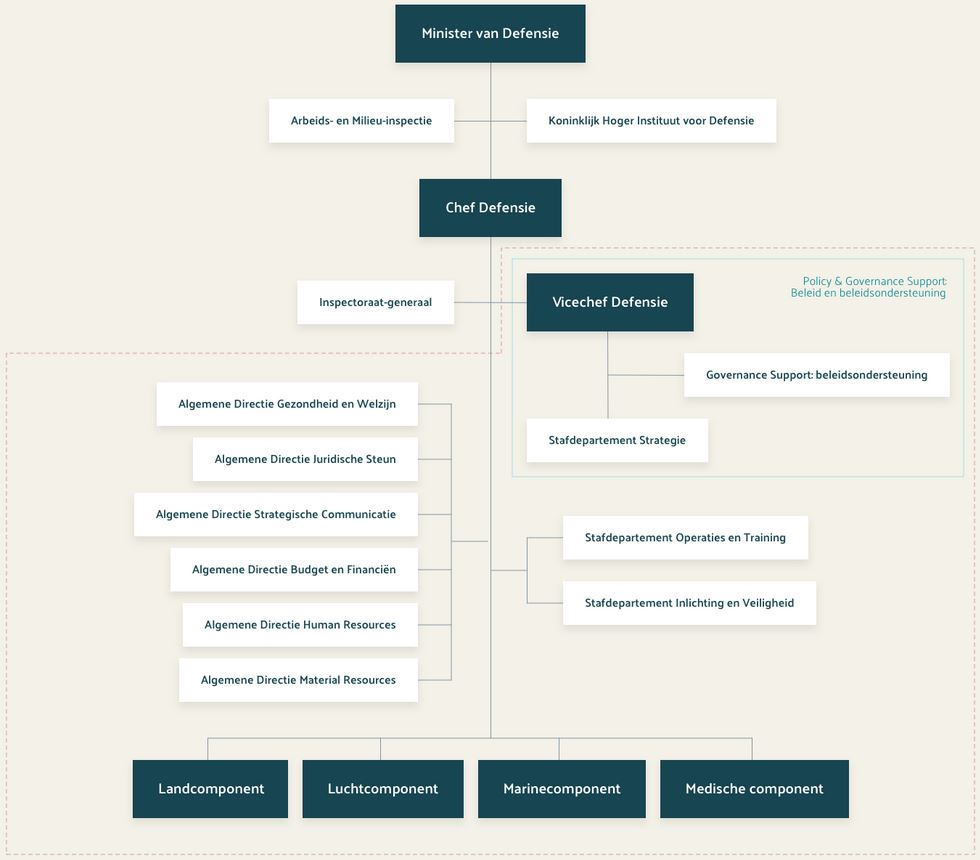
\includegraphics[width=\textwidth]{img/organigram-defensie.png}
    \caption{\label{fig:organigram-defensie}Organigram van Defensie~\autocite{Defensie2022}}
\end{figure}

\subsection{Stageplaats}

Defensie heeft verschillende \glspl{kwartier}, mijn stage vond plaats binnen de \gls{eenheid} \gls{ccvc} op het \gls{kwartier} Majoor Housiau gelegen te Peutie. Zie Figuur~\ref{fig:organigram-ccvc}

\begin{figure}
    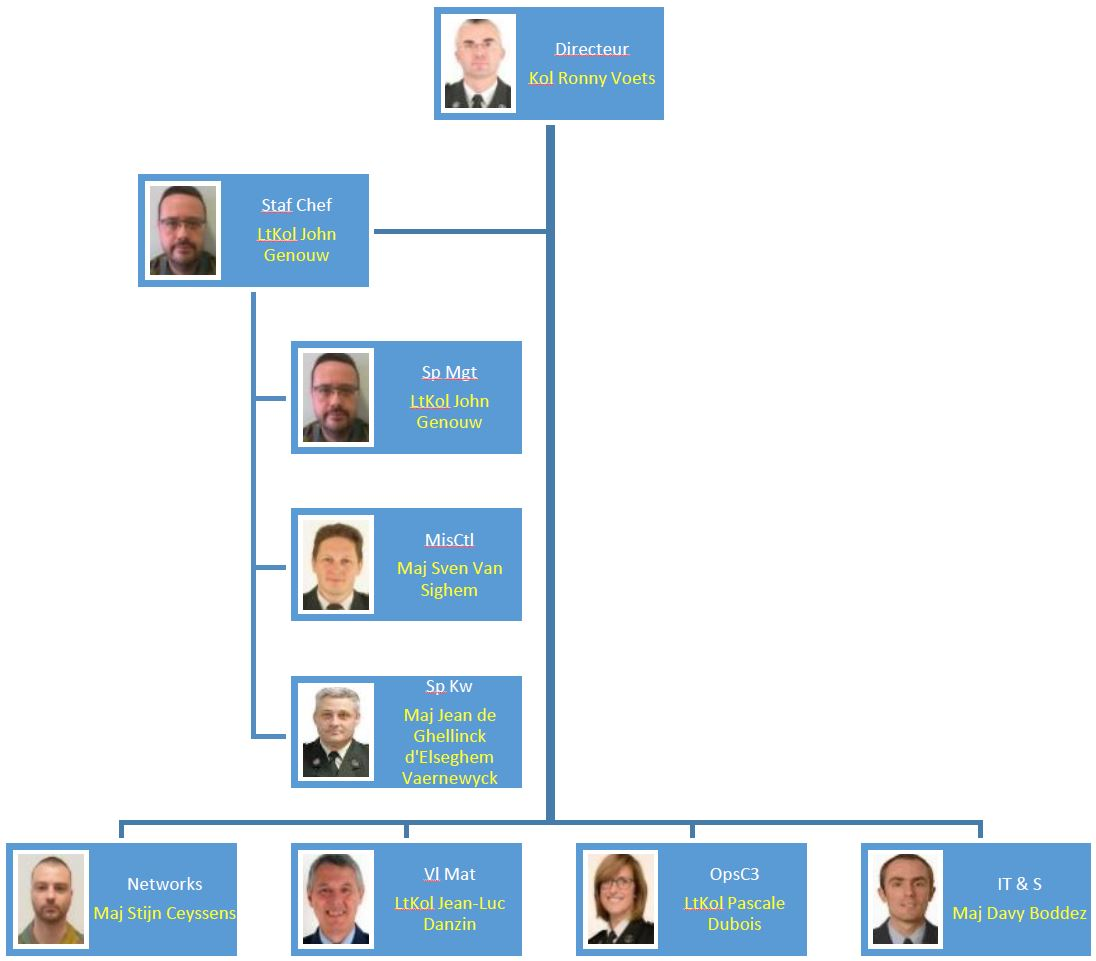
\includegraphics[width=\textwidth]{img/organigram-ccvc.png}
    \caption{\label{fig:organigram-ccvc}Organigram van de \gls{eenheid} \gls{ccvc}~\autocite{Defensie2022a}}
\end{figure}

Mijn stage was bij de afdeling Systems binnen het Departement \gls{its}. Zie figuur~\ref{fig:organigram-its}

\begin{figure}
    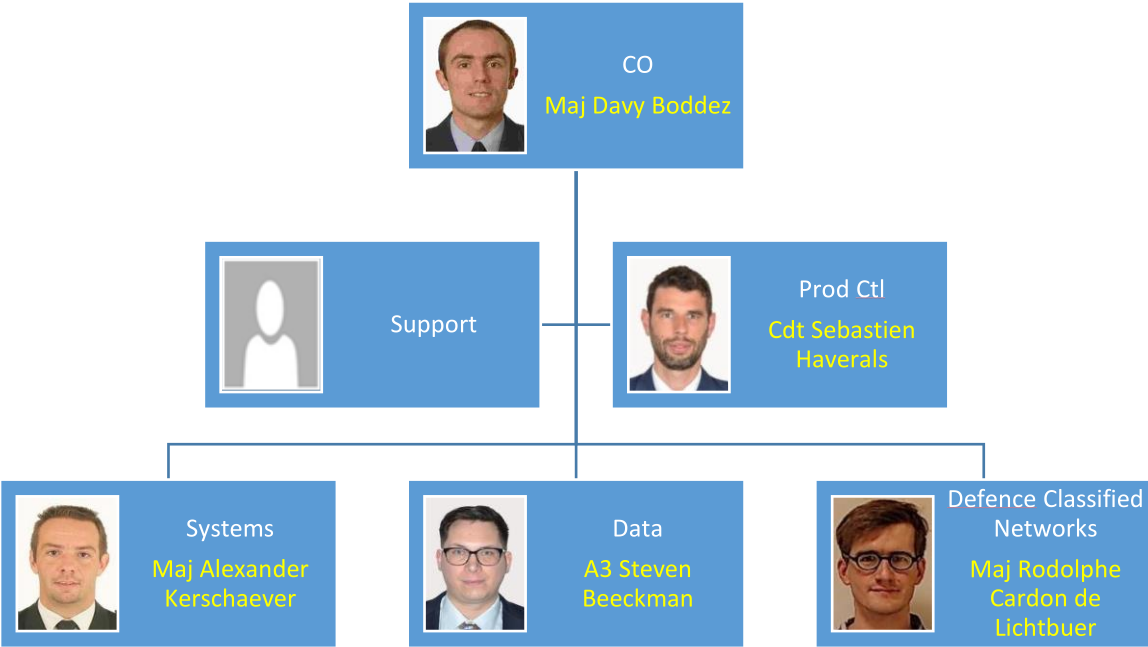
\includegraphics[width=\textwidth]{img/organigram-its.png}
    \caption{\label{fig:organigram-its}Organigram van het departement \gls{its}~\autocite{Defensie2022a}}
\end{figure}

Binnen de afdeling Systems zijn er 6 diensten:

\begin{itemize}
    \item linux
    \item windows
    \item oracle databanken
    \item Microsoft sql server
    \item prodctl
    \item techbu
\end{itemize}

Hoewel ik binnen elke dienst een introductie gekregen heb was miin stage vooral binnen de dienst linux.

Ik heb Defensie gekozen omdat ik ambitie heb om later bij Defensie te gaan werken. Op deze manier kan ik al eens kijken hoe het er aan toe gaat op de werkvloer.